\section{Preprocessing and filtering the dataset}
This work aims to use the hierarchical Stochastic Block Model (hSBM) described before. Data considered in this work have $\sim 11000$ samples as documents and $\sim 60000$ genes as words ($\sim 20000$ if considering only protein-coding genes). The original paper~\cite{gerlach2018network} considers $63$ Wikipedia articles along with $3140$ words. The great amount of data requires some tricks to filter the network and make the computation faster.
Different approaches were tested to pre-process the data. All of them involve the quantities defined in chapter~\ref{ch:structure}. The goal is to identify components which can best partition the realizations and, in the meanwhile, isolate the most interesting genes.
 
\paragraph{Low occurrence genes} were selected firstly to approach topic modelling. A $0.5$ threshold was set on occurrence. This method selects genes that appear (have expression greater than zero) only in less than half samples. This approach has got some limitations, for instance, genes that appear everywhere (with occurrence $\simeq 1$) but change their behaviour across realizations are not considered.

\paragraph{Tf-idf (term frequency–inverse document frequency)} should help. This approach doesn't take into account original expression values $n_{ij}$, but a transformed version
\[
n^{new}_{ij}=\frac{n_{i j}}{M_j}\times \left(1-Log\left(o_i\right)\right)
\] which increases the importance of components with small occurrence $o_i$. This is widely used in linguistics to wash out common words. Tf-idf doesn't select or reduce the number of components (genes), which is still an issue. Moreover, the number of link between nodes is no longer an integer so an approximation is necessary and this introduces a bias.

\paragraph{Highly variable} genes can be selected. This is done using the $CV^2$ analysis done in chapter~\ref{ch:scalinglaws}.
\begin{figure}[htb!]
    \centering
    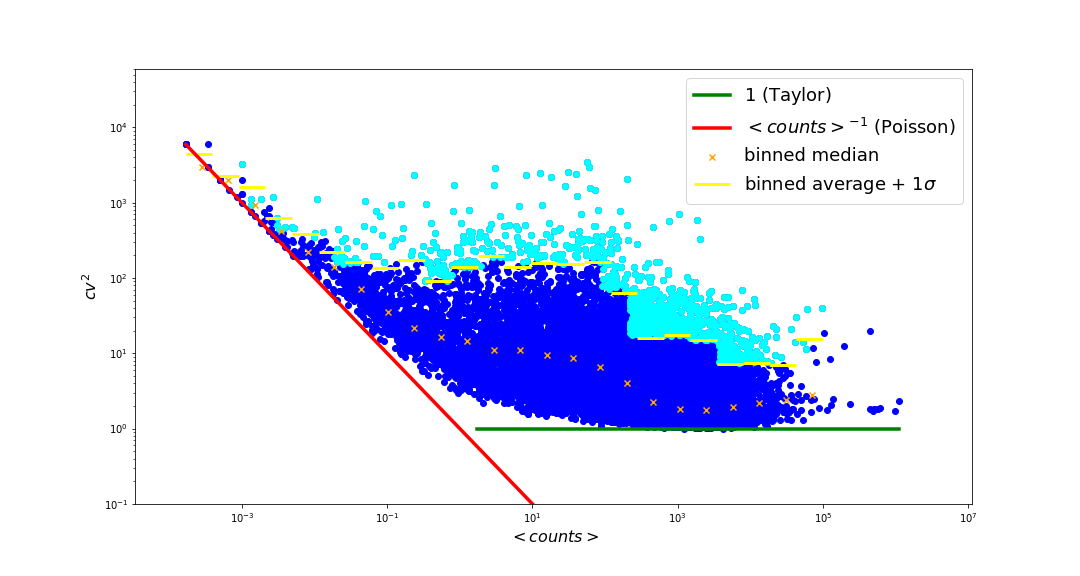
\includegraphics[width=0.8\linewidth]{pictures/topic/cvmean_oversigma.png}
    \caption{Highly variable genes. In \textcolor{pythoncyan}{cyan} genes that are $1 \sigma$ over the average of their bin.}
    \label{fig:topic/cvmean_oversigma}
\end{figure}
Plotting the coefficient of variation versus the mean, one point for each component, one can reveal components that have higher variance than components which, on average, have similar behaviour. Binned averages and variances were estimated. Only genes with a $CV^2$ over a $\sigma$ were considered. This method seems useful to select genes even if the binned average bound is quite noisy.

\paragraph{Distance from boundaries} can be a similar and alternative method to select highly variable genes. In this case, the boundary is both smooth and well-defined.
\begin{figure}[htb!]
    \centering
    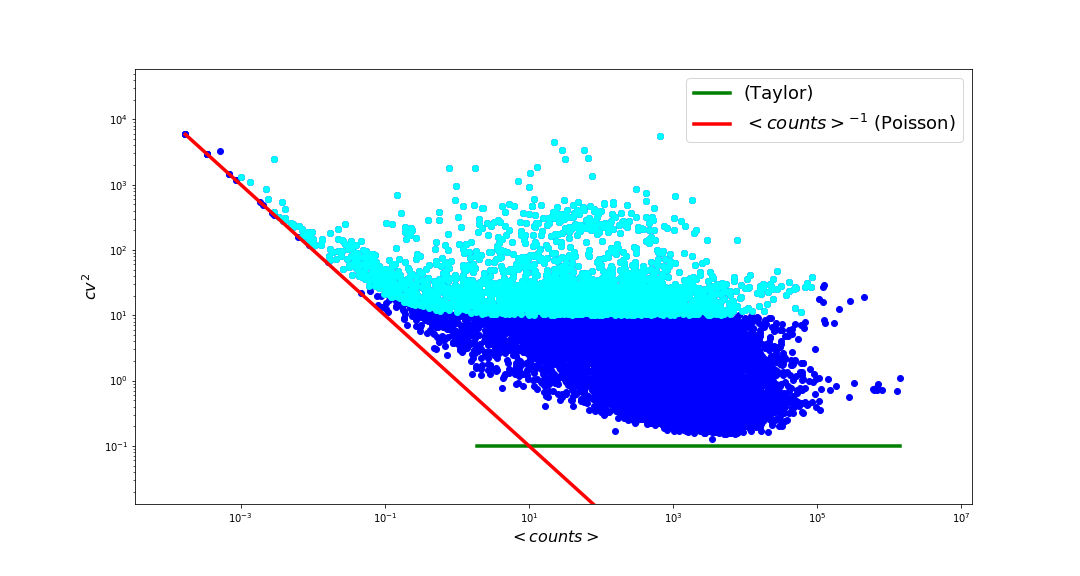
\includegraphics[width=0.8\linewidth]{pictures/topic/cvmean_oversampling.png}
    \caption{In \textcolor{pythoncyan}{cyan} genes which distance from boundaries is greater than $10 CV^2$.}
    \label{fig:topic/cvmean_oversampling}
\end{figure}
The distribution as discussed in~\ref{ch:scalinglaws} has got both a Poisson-like and a Taylor-like boundary. So it is possible to consider only the components that are the most distant from these boundaries. Moreover, these boundaries can be found with a simple null model, as shown in figure~\ref{fig:scalinglaws/gtex/cvmean_loglog_sampling} the sampling model defines the lower bound of the data.
\FloatBarrier
The last two approaches are the ones which lead to the better results, in the following section gene selection was done by getting only highly variables genes.
To reduce the number of documents, samples are picked up uniformly random from a subset of all the available ones.